
\section{Benchmark generation}

Inspired by GQA's pipeline, we generate questions by combining the content of scene graph annotations with question templates~\cite{hudson2019gqa}. Unlike GQA, we use spatio-temporal scene graphs and create new question templates that include a wider variety of temporal reasoning concepts. 

\subsection{Spatio-temporal Scene graphs}

The spatio-temporal scene graphs from Action Genome annotate videos from the Charades dataset about the relationships between a subject and objects over time \cite{ji2020action, sigurdsson2016hollywood}. These videos range in length from 2-194 seconds and are filmed by Amazon Mechanical Turk workers performing skits in their own homes.

\mgm{Delete from this paragraph as space requires - and move to supplementary}
We augment Action Genome's spatio-temporal scene graphs to make the content better suited for quality questions. First, we combined the spatio-temporal scene graph annotations with the Charades action annotations to create a new scene graph with action nodes and denser object and relationship annotations. Next, since the exact second that actions begin and end is often unclear for humans, we add in prior knowledge about actions and adjust the annotations accordingly. For example, it can be assumed that if someone is annotated as "holding a cup" and "putting a cup somewhere" at the same time, they hold the cup first before putting it somewhere. We add in relationship entailments, so that if someone is annotated as "carrying" an object, they are also annotated as "holding" and "touching" it. We took out the attention relationship "looking at" and the negative relationships "not looking at" and "not contacting", and unclear relationships like "unsure" and "other relationship" because those create questions that are difficult for humans to answers. We also simplify the number of objects and actions referred to in a single video, getting rid of references to the same item in the video by multiple phrases. With these and other adjustments, the spatio-temporal scene graphs became densely annotated and referred to objects and events in the video more consistently. This series of edits addressed some of the annotation errors or priors in Action Genome and Charades that lead to non-sensical or incorrect answers. However, some errors in annotations persist and do carry over into our questions. [AMT results preview here?]

After making these corrections, our spatio-temporal scene graphs have 28 objects, 54 relationships, and 157 actions. There are 7,787 training set and 1814 test set scene graphs that fill in question templates.

\subsection{Question Templates}

The second part of the pipeline consists of question templates that each have natural language sentences with tags representing different elements categories in the video, such as in the question "What were they $<$contact relationship$>$?". These tags can be objects, relationships, actions, or phrases that reference a certain part of the video. To increase variety in the dataset, there are multiple natural languages options for each template and the input objects, relationships, and actions are adjusted to be grammatically correct.

\mgm{Moved form experiments section, since we want to talk about diversity in reasoning here}
\textbf{What: } These questions ask what a person was doing. They measure the ability to locate a relationship and determine what object is being used. \mgm{this expl will change if we add in actions}

\textbf{Length: } The length category compares the length of different actions. When generating the questions, we add in a buffer so an action must be annotated as at least 7 seconds longer than another for them to be compared. Length questions are only binary because they are comparisons (e.g. "What did they do for longer $<$action1$>$ or $<$action2$>$) or verification questions (e.g. "Did they do $<$action1$>$ for less time than $<$action2$>$.

\textbf{First and Last: } These questions about the first or last occurrence in the video. 


\textbf{Sequencing: } These questions ask if an action comes before or after another action.

\textbf{Count: } Count questions ask how many times an action occurred, or ask to compare the number of times two actions occur.

\textbf{Exists: } These questions ask if some event occurred



Each template also contains information about the question's structure and the objects, relationships, and actions it references. Finally, each template contains a program that reasons over the spatio-temporal scene graph to automatically generate the answer.

Before adding the question to the dataset, we check that there is no ambiguity in possible answers. We also avoid questions that have common sense combinations ("Are they wearing clothes?"), those that give away the answer ("What did they old while holding a blanket?), and those that are nonsensical ("Were they eating a mirror?").

To generate a question-answer pair, our system combines a spatio-temporal scene graph with these templates by replacing the tags with elements of the corresponding types. For a video where the person is holding a blanket while sitting on a chair, our pipeline would create both questions "What were they holding?" and "What were they sitting on?". Given the scene graph information, we then automatically determine the answers "blanket" and "chair" respectively. We have 27 templates and 251 natural language questions with an answer space of 208. From just these 27 questions, we generate over 133 million question-answer pairs before balancing, with over 90 million unique natural language questions.

\begin{figure}[t]
    \centering
    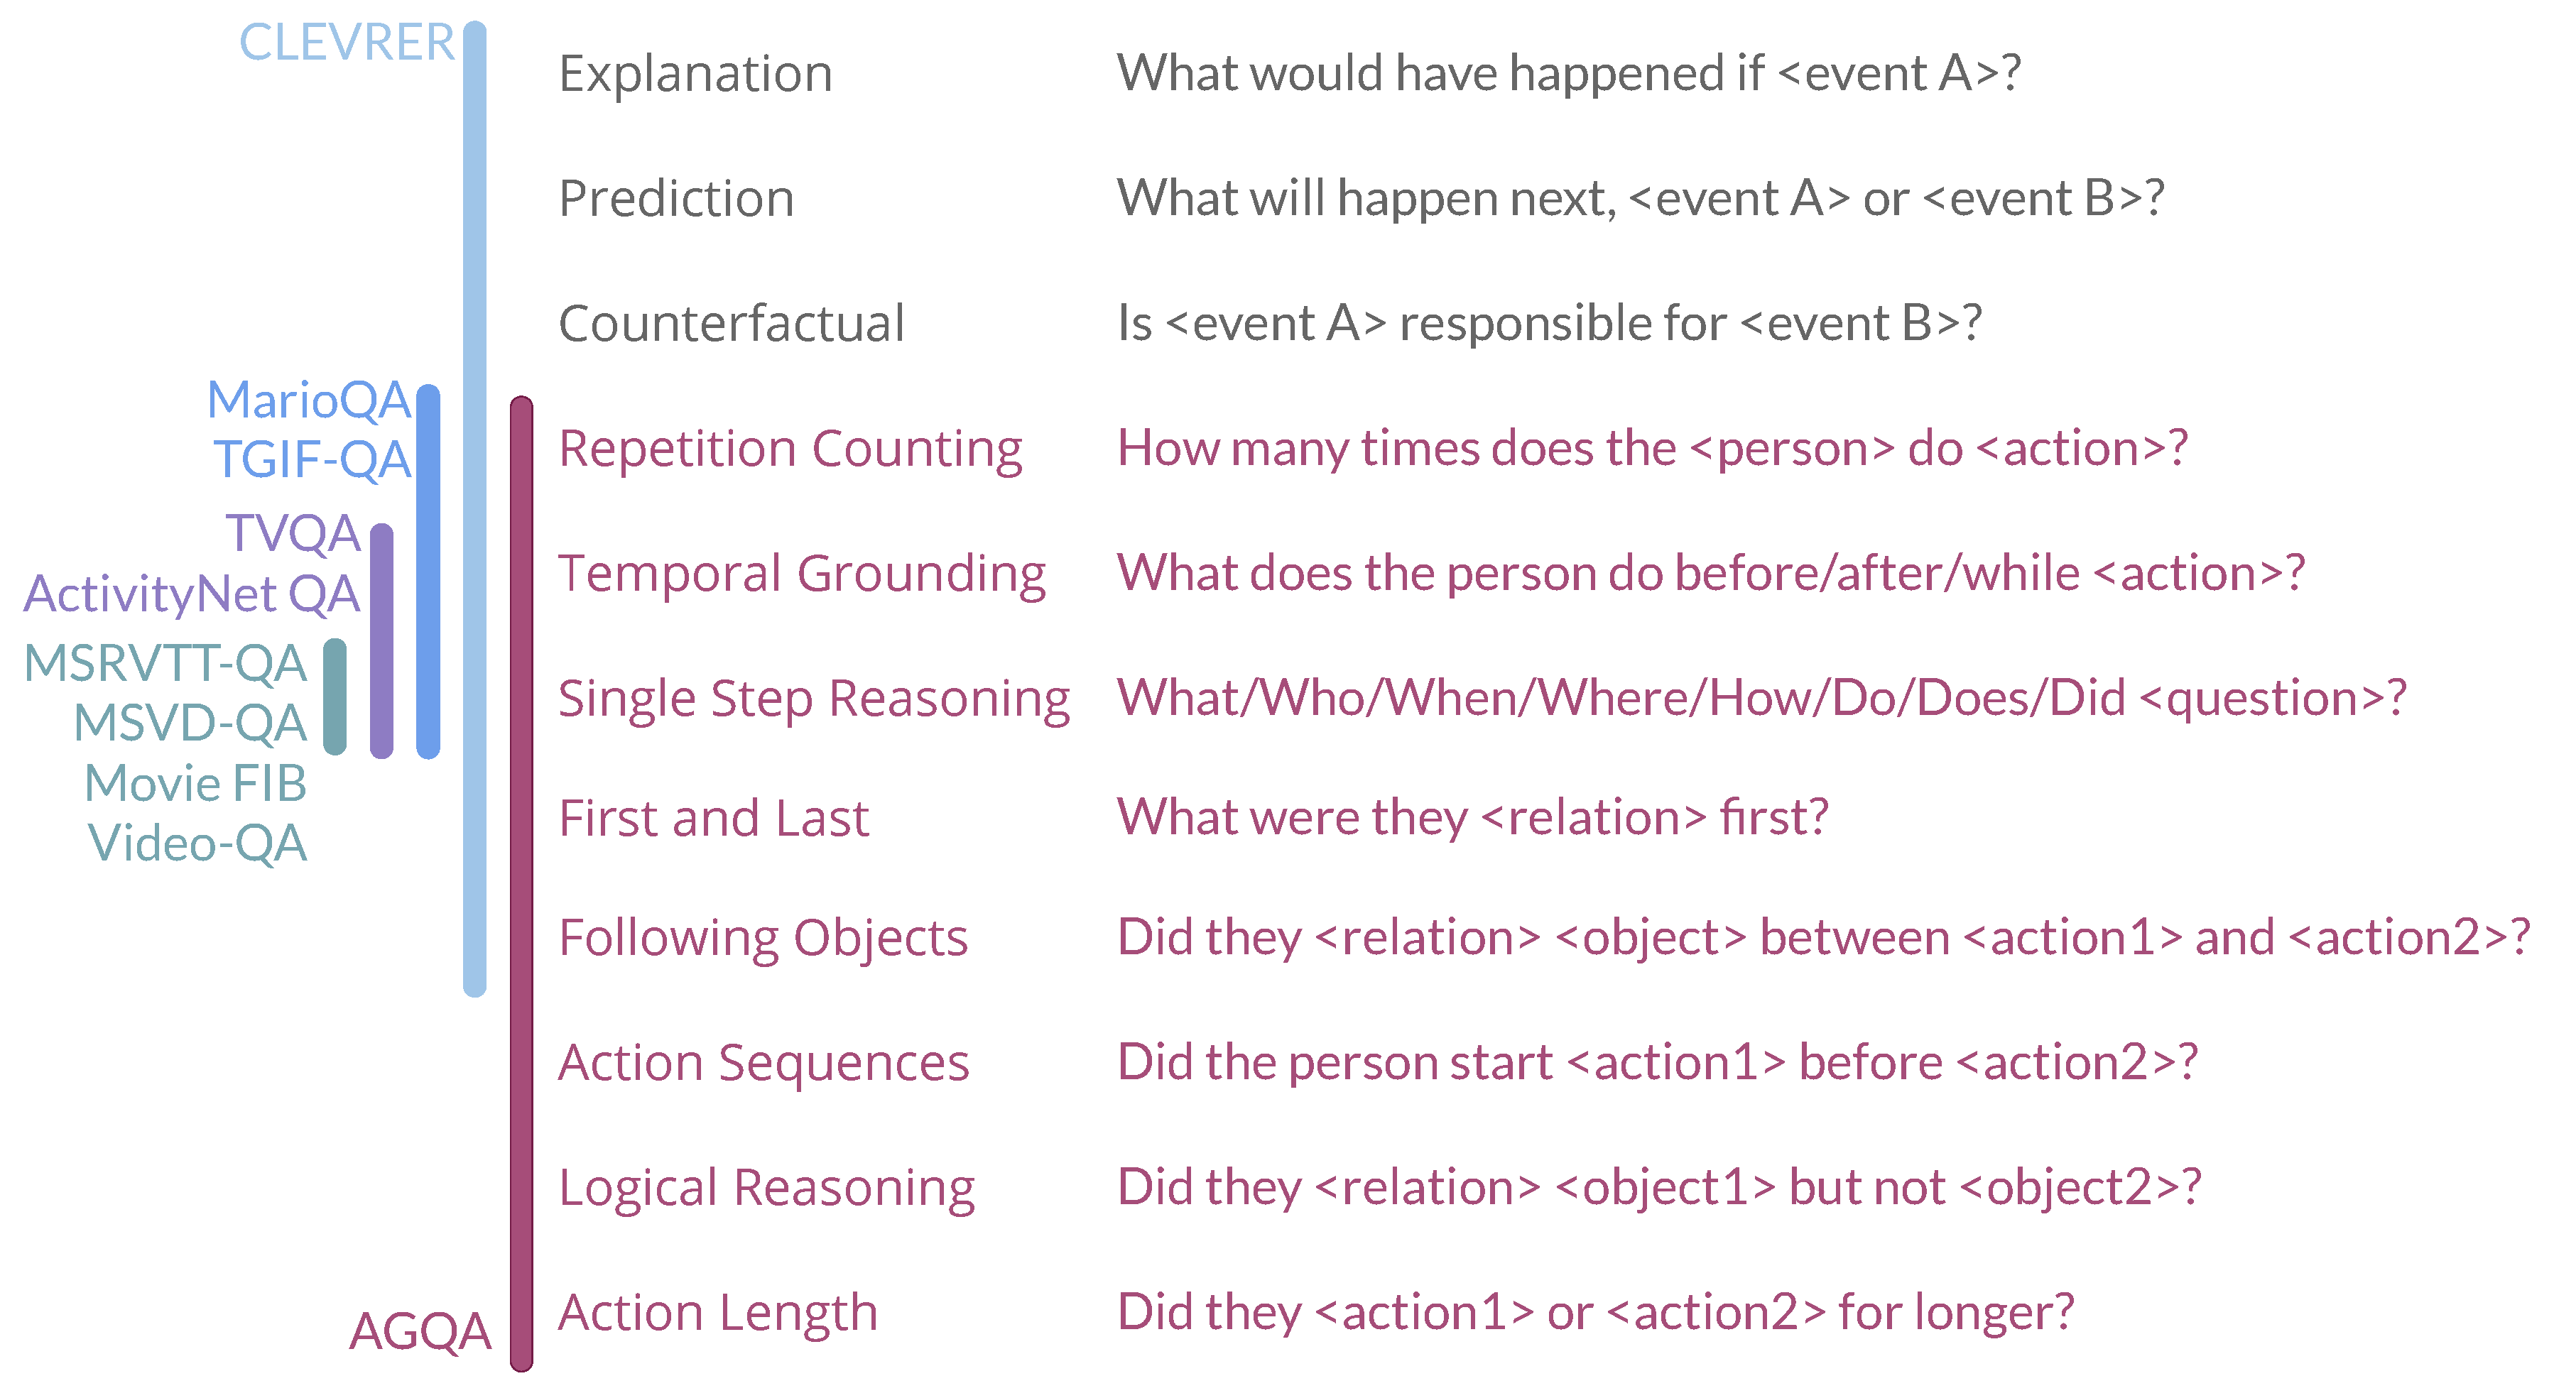
\includegraphics[width=\columnwidth]{figures/questions.pdf}
    \caption{A VideoQA benchmark should be diverse in the spatio-temporal reasoning skills it requires. Since our videos are based on skits, we do not have questions on explanation, prediction, or counterfactual reasoning as does the synthetic dataset CLEVRER~\cite{yi2019clevrer}. However, our questions cover a wider variety of reasoning abilities than other non-synthetic VideoQA benchmarks.}
    \label{fig:questions}
\end{figure}

\subsection{Creating Compositional Reasoning}

Compositional reasoning in questions means that the questions require multiple steps of reasoning to answer. For example, the question "Were they opening a closet or a refrigerator before holding a bag?" requires 1) finding the time at which they hold a bag, 2) shifting attention to before that action, 3) locating when they opened something and 4) determining what object they opened. To generate complex, compositional questions, and to inform a suite of metrics looking specifically at compositional reasoning, we increase compositionality in generated questions in three ways.

First, the question templates themselves can have compositional reasoning. For example, the template "Were they $<$relation$>$ $<$object1$>$ but not $<$object2$>$?" has three reasoning steps 1) searching for if the relation-object1 pair exists, 2) searching for if the relation-object2 pair exists, and 3) a logical operator. 

Second, almost all templates have an optional $<$time$>$ tag that can be filled with a phrase "before/after/while/between $<$action$>$". When this $<$time$>$ tag is filled, the program generating the answer first looks at the indicated frames before figuring out the answer. Therefore, adding in temporal localization phrases adds compositional reasoning steps by first requiring focusing attention on a certain part of the video before continuing with the rest of the template.

Third, $<$object$>$, $<$action$>$, and $<$relation$>$ tags can be filled with both direct and indirect references. An $<$object$>$ could be referred to directly as a "blanket" or indirectly as "the object they threw". An $<$action$>$ can be referred to directly as "eating something" or indirectly as "the longest action". A $<$relation$>$ could be referred to directly as "watching" or indirectly as "the thing they did to the laptop". Since most objects have multiple relations, indirect relationships are less common. Indirect references must be figured out first before answering the rest of the question, so they increase the number of compositional reasoning steps.

Finally, these indirect references and temporal localizations can be combined to create more granular references and even more compositional reasoning steps. Combining a temporal localization with an action indirect reference gets phrases like "before the longest action". When there is ambiguity in an indirect object phrases, such as if they threw multiple things over the course of the video, increased specificity in the indirect references increases complexity (e.g. "the object they threw before going from standing to sitting" or "the object they threw first").

Several other Visual Question Answering benchmarks use compositional reasoning. Our method for creating compositionality is most similar to GQA. However, while GQA uses attributes (e.g. "red") and spatial relations (e.g. "to the left of") as object indirect references, we have temporal localizations, action indirect references, and object indirect references focused on their relationship with the subject \cite{hudson2019gqa}. 

CLEVRER is the VideoQA dataset that thus far most explicitly incorporates compositional reasoning. However, their subjects are somewhat different. They add in compositionality with descriptions of objects (shape, color, material), motion, collision, and temporal ordering. We refer to objects by their interaction with the subject, look at real life videos, and use indirect references in conjunction with other spatio-temporal reasoning skill \cite{yi2019clevrer}.

Of other real-world video question answering sets, TVQA has a similar temporal localization process, but they do not refer to other subjects indirectly, and their questions rely on dialogue and don't have as many reasoning steps built into the template \cite{lei2018tvqa}. All other benchmarks that use temporal localization only ask "What did they do $<$temporal localization$>$?", whereas ours adds in temporal localizations to already complex templates. Finally these real-world VideoQA benchmarks do not systematically add in compositional reasoning in a way that allows it to be specifically measured in metrics. 



\begin{figure}[t]
    \centering
    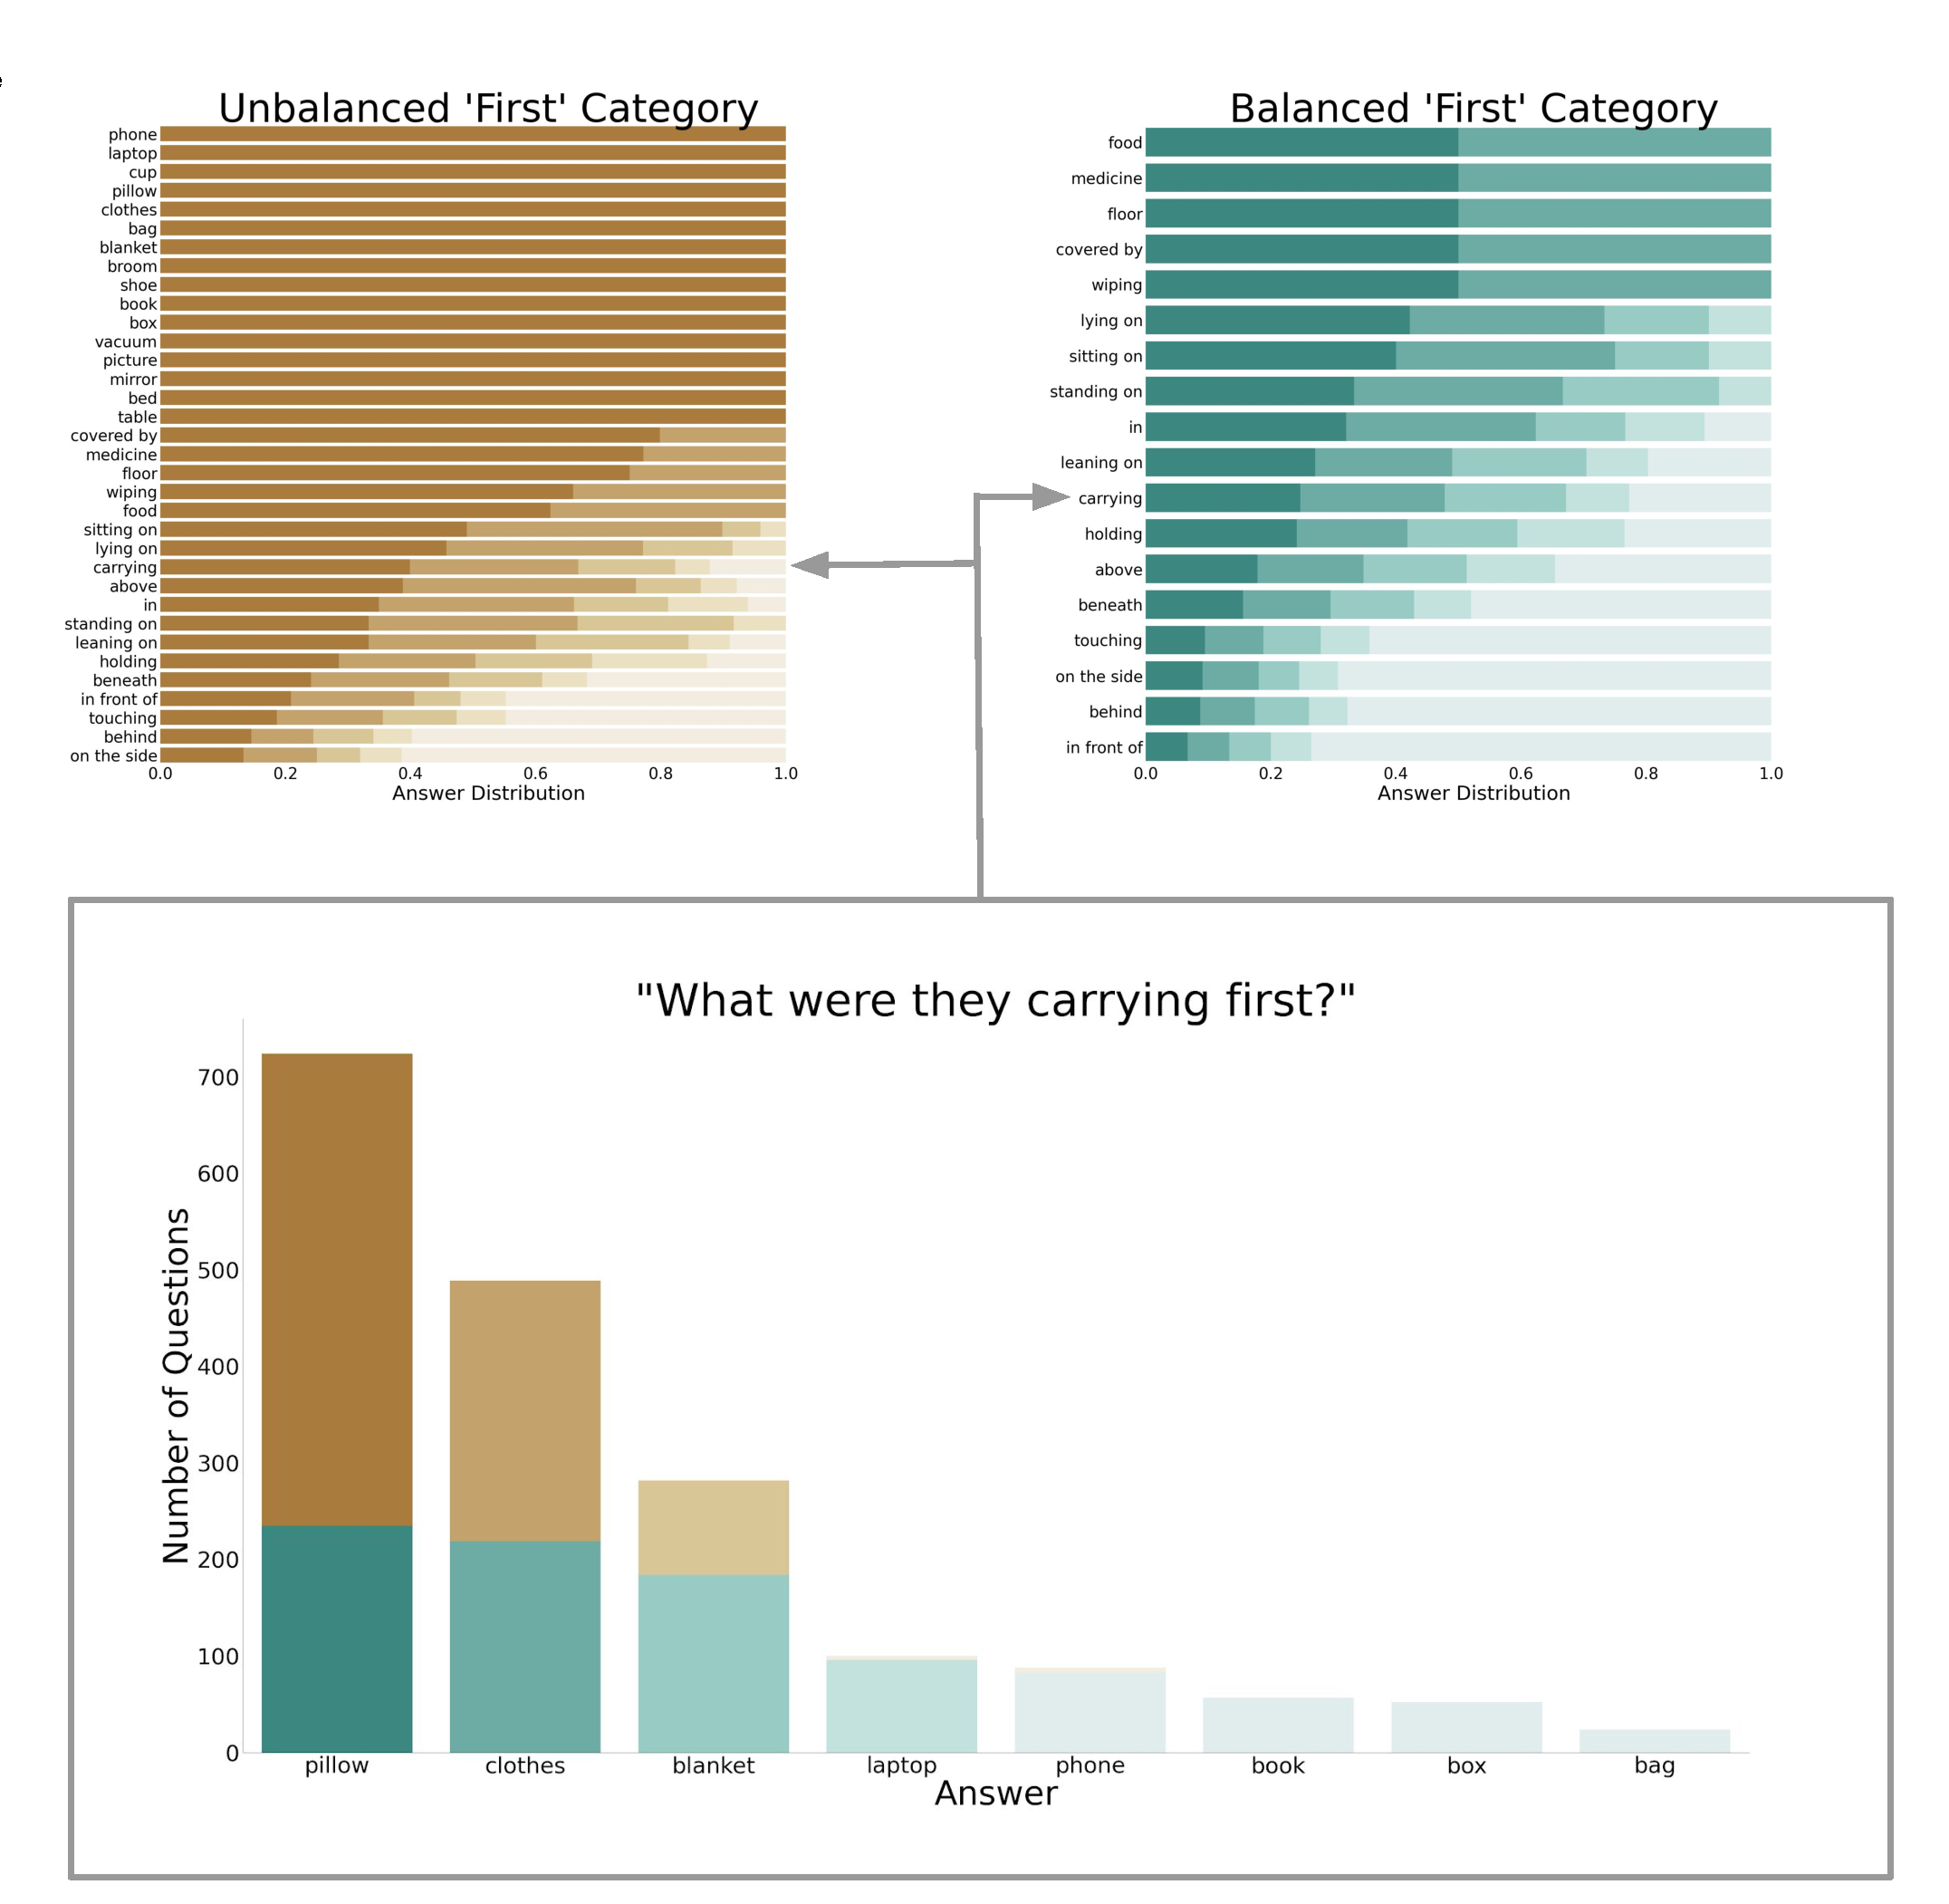
\includegraphics[width=0.95\linewidth]{figures/balance first.pdf}
    \caption{To avoid an artificially easy task, questions should have a diverse set of answers. The bottom row shows the answer distribution for questions that ask "What were they carrying first". In the unbalanced set, the answer "pillow" is correct for nearly 40\% of questions, while after balancing that value drops to 25\%. This balancing effect occurs across all question categories, as seen in the top row.}
    \label{fig:balancefirst}
\end{figure}


\subsection{Balancing}

Machine Learning models are notoriously good at taking advantage of imbalances in the dataset to improve accuracy scores without using the reasoning skills we want to evaluate \cite{hudson2019gqa, goyal2017making, johnson2017clevr, mariani2018bagan, shorten2019survey}. Domains like object detection and image classification have addressed unbalanced datasets by manipulating the image in various ways or using GANs to make categories more balanced \cite{mariani2018bagan, shorten2019survey}. Many VQA datasets contained real world priors exacerbated by human annotation bias, resulting in inflated accuracy scores and a lack of understanding of the actual reasoning abilities of these models~\cite{goyal2017making,hudson2019gqa}. However, balancing answer distributions for the VQA task is difficult for human generated datasets because low control over the content of each question, since often priors in the types of answers each question gets, and because manipulating a natural image in a way that changes the answer of a question is a more difficult task than rotating an image. Previous work reduced imbalances in VQA datasets by reducing skews in the answer distribution \cite{hudson2019gqa, goyal2017making, johnson2017clevr}.

 %For example, in the VQA1.0 dataset, 41\% of answers for questions starting with "What sport is..." were "Tennis". These types of priors meant that models could answer over 50\% of the questions correctly without considering the visual input~\cite{goyal2017making}. Once these issues came to light, some new benchmarks attempted to mitigate these biases. VQA2.0 took many of the questions from VQA1.0 and added a similar picture leading to a different answer. This procedure helped, but was only applied to 71\% of questions due to annotation difficulties. Blind models measured on VQA2.0 could still answer 67\% of binary questions and 27\% of open answer questions correctly without seeing visual input~\cite{hudson2019gqa} \mgm{our open answer blind model is similar... so this point is less salient unless we can bring that down}. 
In the ImageQA task, VQA2.0 took many of the questions from VQA1.0 and added a similar picture leading to a different answer~\cite{goyal2017making}. Synthetic datasets like CLEVR and CLEVRER are able to balance their input because they have tight control over what examples are generated \cite{johnson2017clevr, yi2019clevrer}. The GQA dataset addressed these biases by smoothing the answer distribution by question category. This balancing of the answer distribution retains but reduces the power of real world priors ~\cite{hudson2019gqa}. 

In the Video Question Answering world, CLEVRER creates the most balanced dataset, but it's synthetic generation of videos and limited questions make that an easier task than balancing answer distributions on real-world videos \cite{yi2019clevrer}. On real-world videos, \cite{yu2019activitynet} balances it's yes and no questions and ensures certain categories make up at least 10\% of the dataset. AGQA balances its answer distributions most similarly to GQA that creates smoother distributions at a more granular level than existing real-world VideoQA datasets. 

Our balancing process was adjusted from GQA's. Questions are sorted into global and local categories. Global categories discuss the overall subject of the question (e.g. "counting" or "length"), while local categories are specific to the content of the question (e.g. "counting-throwing some clothes" or "length-running"). Questions also have two answer types, binary and open. Binary questions have two possible answers, such as "Yes/No" or "Before/After". Unlike GQA, we categorize questions that present a choice between two objects, like "Were they to the side of a closet or a bed?", as binary questions as well. Open questions have open-ended answers like "What were they carrying?". 

For binary questions, each local category is balanced such that each possible answer is 50\% likely. For example, for all questions with the base idea "Did they take a blanket from somewhere or go from standing to sitting more times?', half of the questions have "take a blanket from somewhere" as an answer, and half have "go from standing to sitting" as an answer. 

For open questions, we first balanced the global category, then each individual local category. The balancing procedure first truncated 1\% of questions making up the tail of the distribution. \mgm{may want to have a separate algorithm aside to describe this idk. It's a bit of a mouthful} Then, starting with the most popular answer as the "head" it deletes answers in the "head" randomly until either the the proportion of the number of answers in the head and the tail, is less than some number b, or if deleting anymore would change the order of the answer distribution from most frequent to least frequent. Then, the head is expanded to contain an extra answer, and the process repeats. This entire process repeats with b decreasing at every iteration until either half the questions have been deleted, or the most common 20\% of answers made up less than 30\% of all questions. \mgm{Do we need to explain where got the numbers from? It was mostly just experimenting} \mgm{Will be turning this into a figure. }

We then balanced on the structural question types. Query questions are open ended, compare questions compare the qualities of two items, choose questions choose the correct answer from two options, logic questions use logical operators, and verify questions verify if the ideas presented in the question are correct or not. Some templates, especially those with Yes/No answers, had more tags and therefore produced more questions per video. To keep the benchmark challenging with open ended questions, we balanced such that 'query' questions with truly open answers make up half of the dataset.  \mgm{Have a table with the structure, a description, \% before balancing and \% after balancing. Figure for the distribution before and after.}

Finally, we balanced so that for every question with a temporal localization that when added does not change the answer, there is at least one identical question where it does change the answer.

\subsection{Results}
Before balancing, our dataset has over 86.6M question-answer pairs in the training set and over 46.5M question-answer pairs in the test set. After balancing, our dataset has 1.17M question-answer pairs in the training set and 600K question-answer pairs in the test set. Figures of how the distributions changed. We contribute a large, real-world dataset that does compositional reasoning and is balanced to increase difficulty. 
